

\subsection{Overview and class diagram}
\label{sec:overview}

%We give in this section an overview on the main classes. More details about 
%each class and their relations will be explained in the following sections.
%Its core elements are colored in blue. These core elements can also be found in the W3C Provenance Data
%Model. The pattern defined by these classes is very general and can be reused everywhere where provenance is needed. 

% \begin{figure}[ht]
% \centering
% 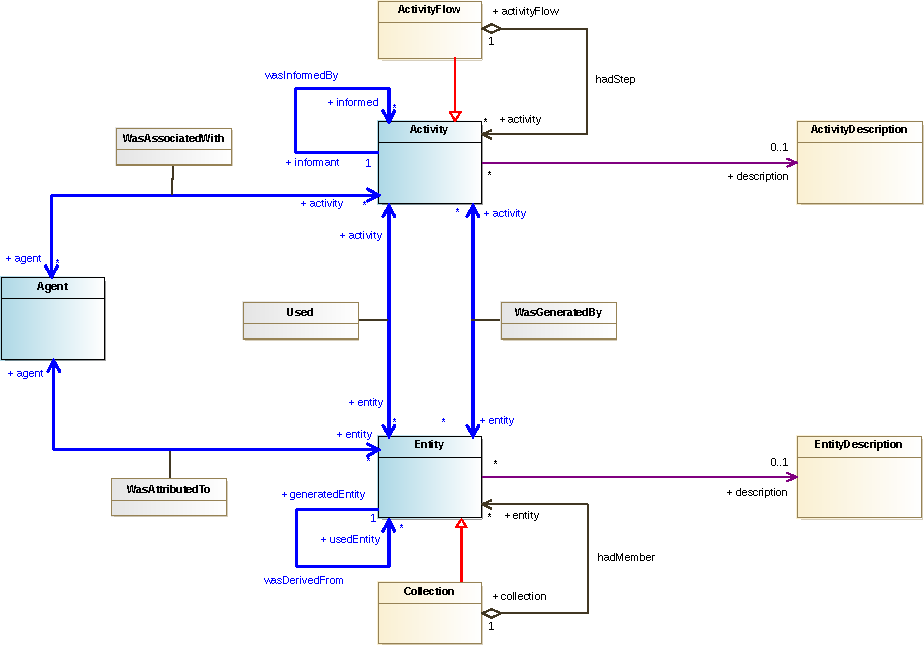
\includegraphics[width=1.0\textwidth]{domain-classdiagram-v2.pdf}
% \caption[Overview: conceptual class diagram of the Provenance Data
% Model]{Overview of the classes for the Provenance DM in a conceptual
% class diagram. The blue classes are core elements. There are a number of
% many-to-many relationships with attached association classes (grey) that may
% contain additional attributes.}
% %Objects in the blue box also appear in the W3C Provenance DM. 
% %Green classes are links to the IVOA Dataset Metadata Model.}
% \label{fig:classdiagram-conceptional}
% \end{figure}

\begin{figure}[hbt]
\centering
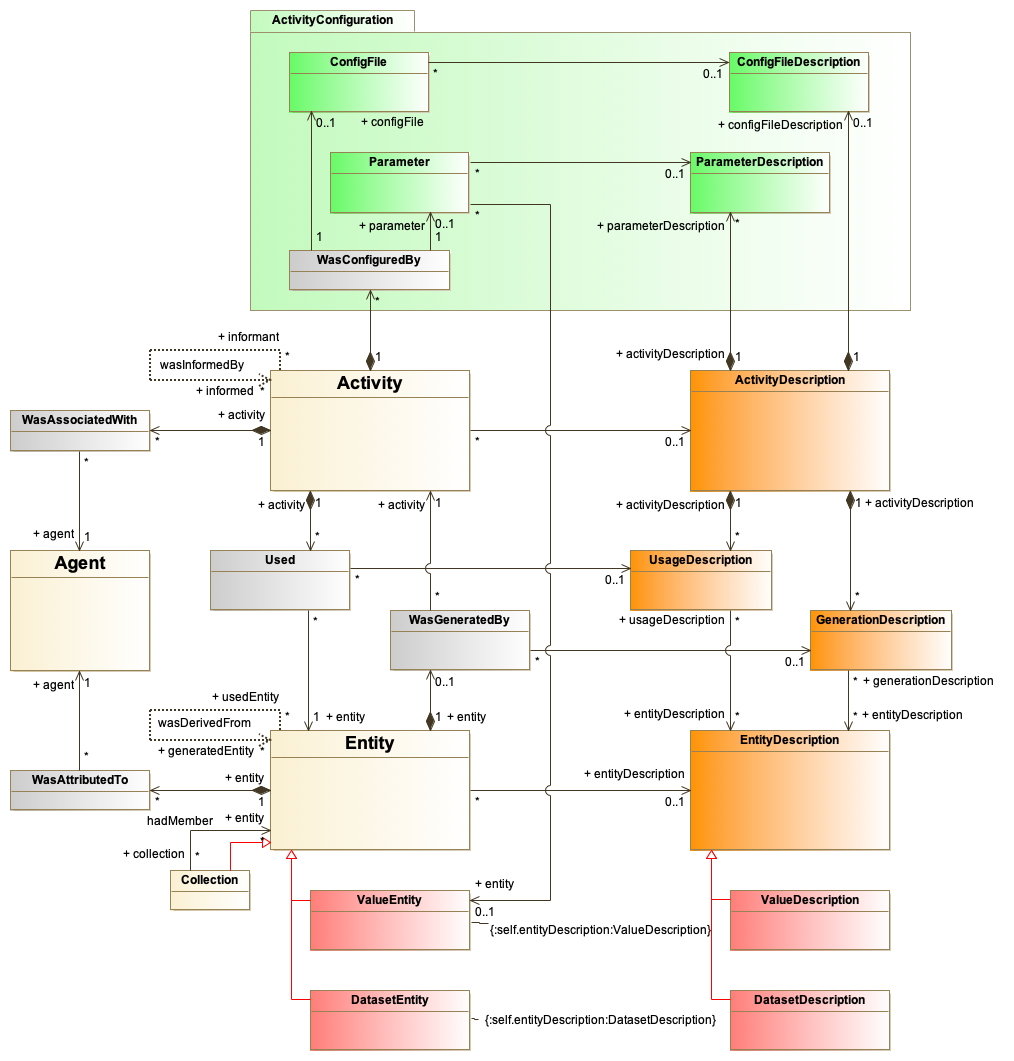
\includegraphics[width=1.0\textwidth]{figures/2019-05-17_IVOAModel_VODML_Overview.png}
\caption[Overview class diagram of the IVOA Provenance Data Model]{Overview class diagram of the IVOA Provenance Data Model. The core part in yellow is based on W3C PROV definitions where relations are shown in grey. It is extended by a Description part (orange), specific types of entities (red) and an optional Activity Configuration package (green). A full diagram with attributes is shown in Section~\ref{sec:fulldiagram}, Figure~\ref{fig:fulldiagram}}
\label{fig:overview}
\end{figure}

The IVOA Provenance DM is based on the the PROV-DM recommendation \citep{std:W3CProvDM} of the World Wide Web Consortium (W3C), that provides the core elements of the model (see Sections~\ref{sec:ent_act} to~\ref{sec:agent+relations}). 
In this context, the provenance of something is a sequence of activities using and generating entities run by agents.

The model includes in addition Description classes (see Section~\ref{sec:descriptions}) to provide information common to several elements; Specific types of Entity classes commonly used in astronomy (see Section~\ref{sec:spec_entities}); and an optional Activity Configuration package (see Section~\ref{sec:configuration}).

The IVOA Provenance DM is a class data model that follows the VO-DML designing rules \citep{std:VODML}. It is represented as a UML class diagram: an overview diagram is shown in Figure~\ref{fig:overview}, and a full diagram with attributes is shown in Appendix~\ref{sec:fulldiagram}, Figure~\ref{fig:fulldiagram}. 


\subsection{Entity-Activity classes}
\label{sec:ent_act}

%\subsubsection{Class diagram}
The core classes and relations of the IVOA Provenance DM are presented in Figure~\ref{fig:coreclasses}.
Traceability (see goal A in Section~\ref{sec:goals}) is enabled by chaining entities and activities, which are the building blocks of the history graph.


\begin{figure}[ht]
\centering
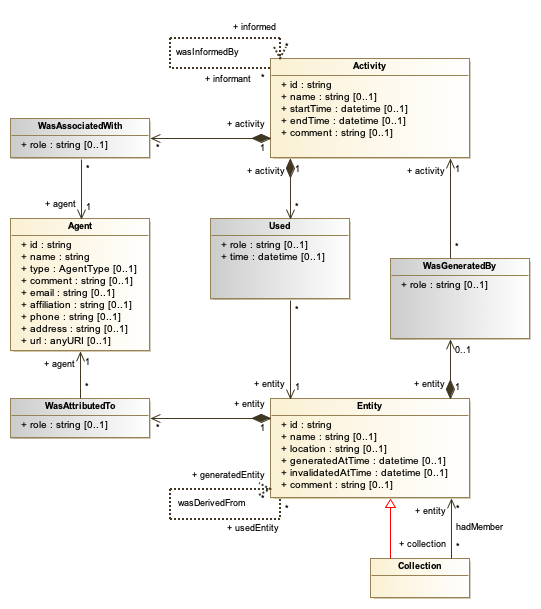
\includegraphics[width=1.0\textwidth]{figures/2019-05-17_CoreModel_VODML.png}
\caption[Core classes and relations]{Core classes and relations. Attributes for these classes are detailed in tables found in Sections~\ref{sec:ent_act} to~\ref{sec:agent+relations}.}
\label{fig:coreclasses}
\end{figure}



\subsubsection{Entity and Collection classes}
\label{sec:Entity}

An \textbf{entity} is a physical, digital, conceptual, or other kind of thing with some fixed aspects (W3C PROV-DM \href{https://www.w3.org/TR/prov-dm/#term-entity}{\S5.1.1}). 

The \class{Entity} class in the model have the attributes given in Table \ref{tab:entity}. 
%If an attribute also exists in the W3C PROV-DM we list its name in the second column.

% 2018-12 commented
%For example: data products such as images, catalogs, calibration data, parameters, configuration files, instrument characteristics, articles, web pages.

Entities in astronomy are usually astronomical or astrophysical datasets in the form of images, tables, numbers, etc. But they can also be log files, files containing system information, any input or output values, environment variables, ambient conditions, or, in a wider sense, observation proposals, scientific  articles, or manuals and other documents. 
Though the focus is on digital entities in this document, entities can also refer to devices such as instruments or tools, that may be linked to digital entities.


\begin{table}[ht]
\small
\tymax  0.5\textwidth
\textbf{\normalsize Entity}\vspace{0.25em}\\
\begin{tabulary}{1.0\textwidth}{llL}
\toprule
\head{Attribute} & \head{Data type} & \head{Description}\\
\midrule
\textbf{id} & string & a unique identifier for this entity\\
name        & string & a human-readable name for the entity\\
%a provenance type, i.e. one of: prov:collection, prov:bundle, prov:plan; or any of the specialized entities defined in Section~\ref{sec:spec_entities} \\
%description\_ref  & foreign key/url & link to \class{EntityDescription}\\
location    & string & a path or spatial coordinates, e.g. a URL, latitude-longitude coordinates on Earth, the name of a place.\\
%value       & prov:value &  & provides a value that is a direct representation of the entity \\
generatedAtTime  & datetime & date and time at which the entity was created (e.g. timestamp of a file)\\
invalidatedAtTime  & datetime & date and time of the destruction, cessation, or expiry of the entity. The entity is no longer available for use (or further invalidation) after invalidation. This does not relate to the validity period of calibration files.\\
comment  &  string & text containing specific comments on the entity\\
%rights      & -- & string & access rights for the entity, values: public, secure or proprietary; see Curation.Rights, RightsType in DatasetDM\\
%\midrule
%$\rightarrow$ description &  & link & link to \class{EntityDescription}\\
%$\rightarrow$ wasAttributedTo & prov:wasAttributedTo & link & link to \class{WasAttributedTo} for linking with a responsible \class{Agent}\\
\bottomrule
\end{tabulary}
\caption[Attributes of the \class{Entity} class]{Attributes of the \class{Entity} class. Attributes in \textbf{bold} must not be null.
%, references are indicated with an arrow ($\rightarrow$). 
%Further project-specific attributes (e.g. size, local path, url, \dots) could be added when relevant for the project (see also Section~\ref{sec:dataset-obscore}). 
% %mireille I would comment this here, because in the model they are in EntityDescrioption while in the implementation one can decide to gather attributes from Entity and EntityDescription together
%Attributes from \class{EntityDescription} (see next section) may appear here as well.
}\label{tab:entity}
\end{table}


%\begin{figure}[ht]
%\centering
%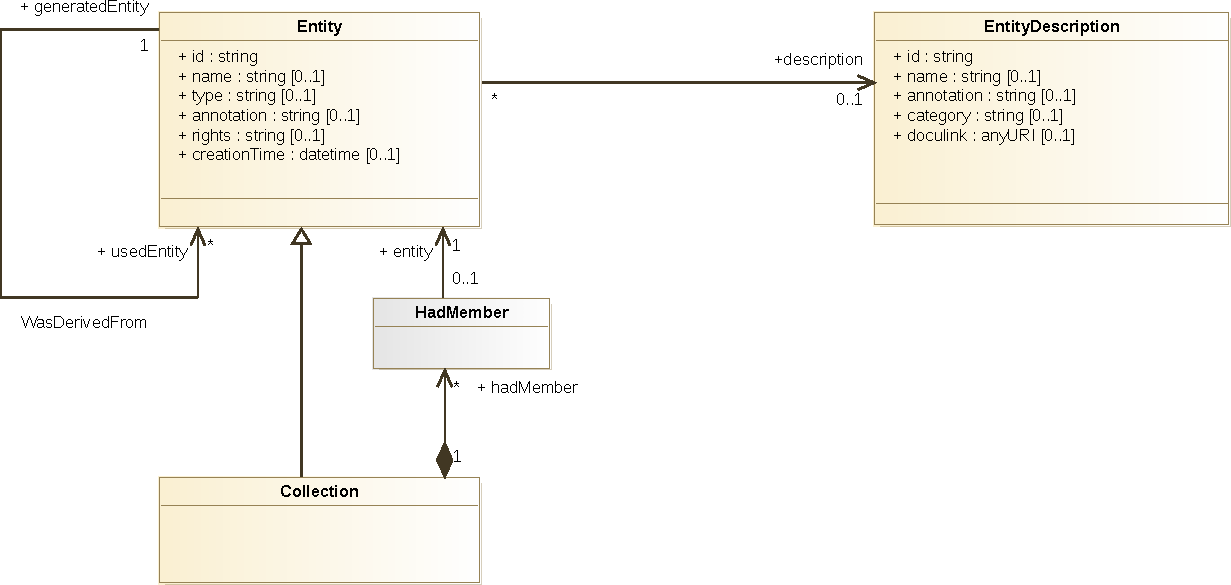
\includegraphics[scale=0.6]{entity-details-v2.pdf}
%\caption[Relations between Entity, EntityDescription and Collection]{The relations between Entity, %EntityDescription and Collection (see Section~\ref{sec:collection}). 
%Links to the Dataset class from the Dataset Metadata Model are described in Section~\ref{sec:dmlinks}.}
%\label{fig:entity-details}
%\end{figure}

% 2018-12 commented
%The VO concept closest to \class{Entity} is the notion of \class{Dataset}, which
%could mean a single table, an image or a collection of them. The Dataset
%Metadata Model \citep{std:DatasetDM} specifies that a \class{Dataset} as ``a file or
%files which  are considered to be a single deliverable''.  Most attributes of
%the \class{Dataset} class can be mapped directly to attributes of the
%\class{Entity} class, see the mappings of 
%Table~\ref{tab:datasetmapping} in Section~\ref{sec:dmlinks}.



A \textbf{collection} is an entity that provides a structure to some constituents that must themselves be entities (W3C PROV-DM \href{https://www.w3.org/TR/prov-dm/#term-collection}{\S5.6.1}). These constituents are said to be member of the collections. They are connected in the model with a \class{hadMember} relation.

%An additional class \class{CollectionDescription} is only 
%needed if it has different attributes than 
%the \class{EntityDescription}. This class should therefore only be introduced if a use case requires it.

%\TODO{Find a really strong use case for Collections to convince everyone that they are useful/needed.}


\subsubsection{Activity class}
\label{sec:activity}

An \textbf{activity} is something that occurs over a period of time and acts upon or with entities; it may include consuming, processing, transforming, modifying, relocating, using, or generating entities (W3C PROV-DM \href{https://www.w3.org/TR/prov-dm/#term-Activity}{\S5.1.2}). 

The \class{Activity} class in the model have the attributes given in Table \ref{tab:activity}. 

% 2018-12 commented
%For example: data acquisition like observation, simulation; regridding, fusion, calibration steps, reconstruction; edition, publication, release of data.

Activities in astronomy include all steps from obtaining data to the reduction
of  images and production of new datasets, such as image calibration, bias
subtraction, image stacking, light curve generation from a number of
observations, radial velocity determination from spectra, post-processing steps
of simulations, etc.


%\begin{figure}[ht]
%\centering
%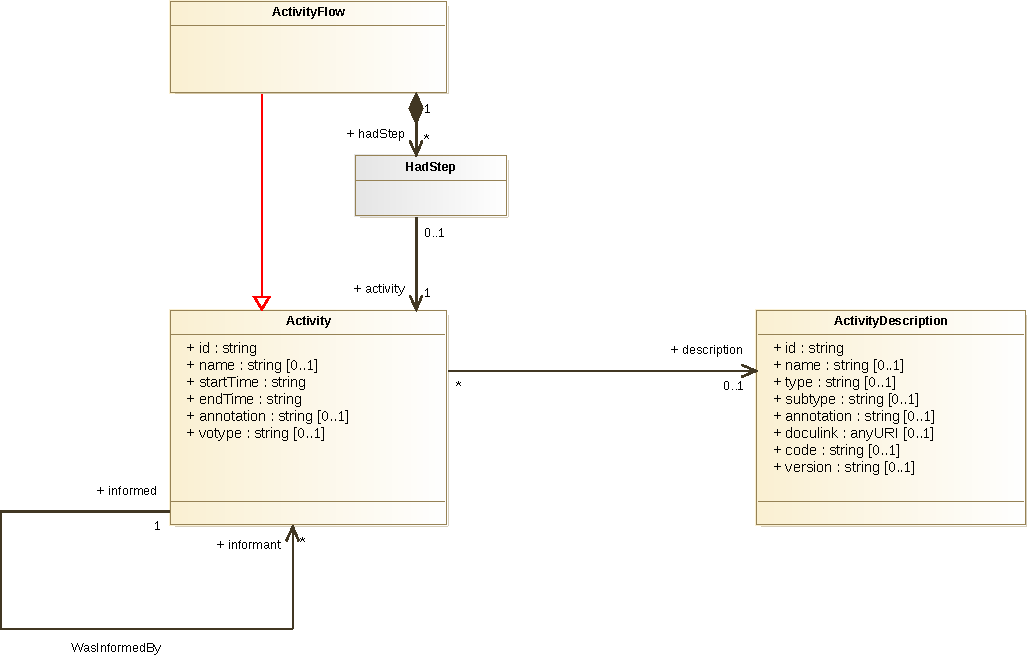
\includegraphics[scale=0.7]{activity-details.pdf}
%\caption[Details for Activity, ActivityDescription and ActivityFlow]{Details for Activity, %ActivityDescription and ActivityFlow (Sections~\ref{sec:activity} and \ref{sec:activityflow}).
%}
%\label{fig:activity-details}
%\end{figure}

\begin{table}[ht]
\small
\tymax  0.5\textwidth
\textbf{\normalsize Activity}\vspace{0.25em}\\
\begin{tabulary}{1.0\textwidth}{llL}
\toprule
\head{Attribute}  & \head{Data type} & \head{Description}\\
\midrule
\textbf{id}  & string & a unique id for this activity\\
name         & string & a human-readable name (to be displayed by clients)\\
startTime    & datetime & start of an activity\\
endTime      & datetime & end of an activity\\
% startTime and endTime are not strictly required -- and in case of a reproducible activity
% they are meaningless. Therefore, I removed the bf here.
% mireille :  I do not agree for this change by Ole : They can be unknown but they must be mandatory in order to allow to query on time for an activity, and to tell the execution order. 
% ole so what should I put there if the time is not known? And what is the use case of using the temporal execution order instead of the logical one (following the provenance links used/wasgeneratedby)?
comment      & string & text containing specific comments on the activity\\
%status &  & string & can be used to describe the terminal status of the activity (e.g. completed, aborted, error...)\\
%votype & string & can be either ``activity'' or ``activityFlow''\\
%, used to differentiate between these two class types, if ``activityFlow'' is not implemented as an extra class (and in W3C compatible serializations)\\
%\midrule
%$\rightarrow$ description &  & link & link to \class{ActivityDescription}\\
%$\rightarrow$ wasAssociatedWith & prov:wasAssociatedWith  & link & link to \class{WasAssociatedWith} for linking with a responsible \class{Agent}\\
\bottomrule
\end{tabulary}
\caption[Attributes of the \class{Activity} class.]{Attributes of the \class{Activity} class. Attributes in \textbf{bold} must not be null.}\label{tab:activity}
%, references are indicated with an arrow ($\rightarrow$).}
\end{table}

% 2018-12 commented
%An Activity can be seen as the node that helps to discover the progenitors of a dataset and any additional information on its generation.



\subsection{Entity-Activity relations}
\label{sec:entity-activity-relations}

Each entity is usually a result of an activity, expressed by a link from the entity to its generating activity, and can be used as input for (many) other activities.
Thus the information on whether data is used as input or was produced as output of some activity is given by the \emph{relations} between activities and entities.
Tracking those relations answers one of the main objective of the model (see goal A in Section~\ref{sec:goals}).


\subsubsection{Used class}

\textbf{Usage} is the beginning of utilizing an entity by an activity. Before usage, the activity had not begun to utilize this entity and could not have been affected by the entity (W3C PROV-DM \href{https://www.w3.org/TR/prov-dm/#term-Usage}{\S5.1.4}).

Usage is implemented in the model by a class \class{Used} that connects \class{Activity} to \class{Entity} and contains the attributes in Table~\ref{tab:used}.

For example, an activity ``calibration'' used entities with the roles ``calibration data'' and ``raw images''.

\begin{table}[ht]
\small
\tymax  0.5\textwidth
\textbf{\normalsize Used}\vspace{0.25em}\\
\begin{tabulary}{1.0\textwidth}{llL}
\toprule
\head{Attribute} & \head{Data type} & \head{Description}\\
\midrule
%\multicolumn{4}{@{}l}{References}\\
%\midrule
%$\rightarrow$ \textbf{activity} & prov:activity & link & link to an \class{Activity} instance\\
%$\rightarrow$ \textbf{entity} & prov:entity & link & link to an \class{Entity} instance\\
%$\rightarrow$ description  &  & link & link to the corresponding \class{UsedDescription}, if existing\\
%\midrule
%\textbf{id} & prov:id  & string & an identifier for this relation\\
role  & string   & function of the entity with respect to the activity\\
time  & datetime & time at which the usage of an entity started\\
\bottomrule
\end{tabulary}
\caption[Attributes of the \class{Used} relation class]{Attributes of the \class{Used} relation class.}
%References in the data model are indicated with an arrow ($\rightarrow$). Attributes in \textbf{bold} must not be null.}
\label{tab:used}
\end{table}

The \attribute{time} of the usage can be specified, and must be between the \attribute{startTime} and the \attribute{stopTime} of the corresponding activity.

The \class{Used} class is closely coupled to the \class{Activity} by a composition (see \ref{sect:Composition}). 
Any given entity can be used by more than one activity.
%If an activity is deleted, then the corresponding \class{Used} relations need to be removed as well. The entities that were used still remain, since they may have been used for other activities as well. The multiplicity is * between \class{Used} and \class{Entity}, because an entity can be used more than once (by different activities).


\subsubsection{WasGeneratedBy class}

\textbf{Generation} is the completion of production of a new entity by an activity. This entity did not exist before generation and becomes available for usage after this generation (W3C PROV-DM \href{https://www.w3.org/TR/prov-dm/#term-Generation}{\S5.1.3}).
        
Generation is implemented in the model by a class \class{WasGeneratedBy} that connects \class{Entity} to \class{Activity} and contains the attributes in Table~\ref{tab:used}.

For example, the entity ``raw\_image.fits'' wasGeneratedBy the activity ``observation'' with the role ``raw image''.

\begin{table}[ht]
\small
\tymax  0.5\textwidth
\textbf{\normalsize WasGeneratedBy}\vspace{0.25em}\\
\begin{tabulary}{1.0\textwidth}{llL}
\toprule
\head{Attribute} & \head{Data type} & \head{Description}\\
\midrule
%\multicolumn{4}{@{}l}{References}\\
%\midrule
%$\rightarrow$ \textbf{entity} & prov:entity & link & link to an \class{Entity} instance\\
%$\rightarrow$ \textbf{activity} & prov:activity & link & link to an \class{Activity} instance\\
%$\rightarrow$ description  &  & link & link to the corresponding \class{WasGeneratedByDescription}, if existing\\
%\midrule
%\textbf{id} & prov:id  & string & an identifier for this relation\\
role   &  string   &  function of the entity with respect to the activity\\
%time & prov:time & datetime & time at which the generation of an entity is finished\\
\bottomrule
\end{tabulary}
\caption[Attributes of the \class{WasGeneratedBy} relation class]{Attributes of the \class{WasGeneratedBy} relation class.}
%References in the data model are indicated with an arrow ($\rightarrow$). Attributes in \textbf{bold} must not be null.}
\label{tab:wasgeneratedby}
\end{table}

As the \class{Entity} class has an attribute \attribute{generatedAtTime}, there is no additional time attribute in this relation.

The \class{WasGeneratedBy} relation is closely coupled with the \class{Entity} via a composition (see \ref{sect:Composition}). 
%, as indicated in Figure~\ref{fig:coreclasses} by a filled diamond. If an entity is deleted, then its \class{WasGeneratedBy} relation must be deleted as well. There is a multiplicity * between \class{Activity} and \class{WasGeneratedBy}, because an activity can generate many entities. However, 
An entity can be generated by only one activity, so the multiplicity is 1 or 0 between \class{Entity} and \class{WasGeneratedBy}.


\subsubsection{Roles in Entity-Activity relations}
\label{sec:roles}

%Each activity generally assign specific roles to each input or output entity. 
The \attribute{role} of an entity within an activity should be provided. 
Roles in Entity-Activity relations are free text attributes.
%, but may contain reserved words in the future to foster interoperability.
%, except for predefined words listed in a dedicated vocabulary webpage.

The \attribute{role} cannot be an attribute of the \class{Entity} class, since the same entity (e.g. a specific file containing an image) may play different roles with different activities. 
%If this is not the case, if the image can only play the same role everywhere, only then it can be an intrinsic property of the entity.

In some cases the role is mandatory to distinguish two input entities. For example, an activity for dark-frame subtraction requires two input images. But it is very important to know which of the images is the raw image and which one fulfils the role of dark frame.

Several entities may play the same role for an activity. For example, many image entities may be used as science-ready-images for an image stacking process. 


% \subsection{Derivation and Communication}

% 2019-05 change to optional
% This section is non-normative but provides important definitions concerning entities, activities and their relations.

% One objective of the model is to be able to visualize independently the flow of entities, e.g. a dataflow, and the flow of activity as it occurred, which may be the result of the execution of a workflow (see goal A in Section~\ref{sec:goals}). 
% Definitions are thus required for dedicated relations between two entities and between two activities.

% Such relations do not need a priori specific classes or tables in an implementation, but provide a way to expose partial information already described by the implemented chains WasGeneratedBy-Activity-Used (Derivation) or Used-Entity-WasGeneratedBy (Communication), where the activity or the entity may be an empty instance.




\subsubsection{WasDerivedFrom relation}

A \textbf{derivation} is a transformation of an entity into another, an update of an entity resulting in a new one, or the construction of a new entity based on a pre-existing entity (W3C PROV-DM \href{https://www.w3.org/TR/prov-dm/#term-Derivation}{\S5.2.1}).

Derivation is an optional relation \class{wasDerivedFrom} in the model, that connects an instance of \class{Entity} to another instance.
%and contains the attributes in Table~\ref{tab:wasderivedfrom}.
%A Derivation may also have relations to \class{Activity}, \class{Used} and \class{WasGeneratedBy} instances.

For example, the entity ``calibrated\_image.fits'' wasDerivedFrom the entity ``raw\_image.fits''
%, with a relation to the activity ``calibration'' and the corresponding Used and WasGeneratedBy instances.

This relation makes it possible to visualize independently the flow of entities, e.g. a dataflow. It does not need a priori a specific class or table in an implementation, but it provides a way to expose partial information that follow the general chain \class{WasGeneratedBy-Activity-Used} where the activity may be an empty instance because it is unknown or irrelevant.


% 2019-01 commented
% \begin{table}[ht]
% \small
% \tymax  0.5\textwidth
% \textbf{\normalsize WasDerivedFrom}\vspace{0.25em}\\
% \begin{tabulary}{1.0\textwidth}{@{}lp{3cm}L@{}}
% \toprule
% \head{Attribute} & \head{Data type}   & \head{Description}\\
% \midrule
% $\rightarrow$ \textbf{generatedEntity} & link      & link to the \class{Entity}\\
% $\rightarrow$ \textbf{usedEntity}      & link      & link to the progenitor \class{Entity}, from which the generatedEntity was derived\\
% \midrule
% %\textbf{id} & string & an identifier for this relation\\
% activity         & string            & id of the underlying \class{Activity} if it is unique\\
% generation       & string            & id of the underlying \class{WasGeneratedBy} relation\\
% usage            & string            & id of the underlying \class{Used} relation\\
% \bottomrule
% \end{tabulary}
% \caption[Attributes of the \class{WasDerivedFrom} relation class]{Attributes of the
% \class{WasDerivedFrom} relation class. References in the data model are indicated with an arrow ($\rightarrow$). Attributes in \textbf{bold} must not be null.}\label{tab:wasderivedfrom}
% \end{table}


\subsubsection{WasInformedBy relation}

\textbf{Communication} is the exchange of information (some unspecified entity) by two activities, one activity using some entity generated by the other (W3C PROV-DM \href{https://www.w3.org/TR/prov-dm/#term-Communication}{\S5.1.5}).

Communication is an optional relation \class{wasInformedBy} in the model, that connects an instance of \class{Activity} to another instance.

For example, the activity ``calibration'' wasInformedBy the activity ``pipeline''.

This relation makes it possible to visualize independently the flow of activities as they occurred, which may be the result of the execution of a workflow. It does not need a priori a specific class or table in an implementation, but it provides a way to expose partial information that follow the general chain \class{Used-Entity-WasGeneratedBy} where the entity may be an empty instance because it is unknown or irrelevant.


% \paragraph{WasPartOf.}
% This relation, taken form the ProvONE ontology, enables the specification of the structure of \class{Activity} instances in that a parent \class{Activity} has child \class{Activities}. Such a structure can help to describe the steps of a pipeline, or a workflow.

% \begin{table}[ht]
% \small
% \tymax  0.5\textwidth
% \textbf{\normalsize WasPartOf}\vspace{0.25em}\\
% \begin{tabulary}{1.0\textwidth}{@{}lp{3cm}L@{}}
% \toprule
% \head{Attribute} & \head{Data type}   & \head{Description}\\
% \midrule
% %id               & string            & a unique id\\
% $\rightarrow$ \textbf{parent} & link      & link to the parent \class{Activity}, e.g. a workflow\\
% $\rightarrow$ \textbf{child}      & link      & link to the child \class{Activity}\\
% %activity         & string            & id of the generation \class{Activity}\\
% %generation       & string            & id of the \class{WasGeneratedBy} relation\\
% %usage            & string            & id of the \class{Used} relation\\
% \bottomrule
% \end{tabulary}
% \caption[Attributes of the \class{WasPartOf} relation]{Attributes of the \class{WasPartOf} relation.
% }\label{tab:waspartof}
% \end{table}



\subsection{Agent and relations to Agent}
\label{sec:agent+relations}

A contact information is needed in case more information about a certain activity or entity is required, but also in order to know who was involved and to fulfil the Acknowledgement objective (see goal B in Section~\ref{sec:goals}).
%, so that proper credits are given to the right people/projects. 


\subsubsection{Agent class}
\label{sec:agent}

An \textbf{agent} is something that bears some form of responsibility for an activity taking place or for the existence of an entity (W3C PROV-DM \href{https://www.w3.org/TR/prov-dm/#term-agent}{\S5.3.1}).

The \class{Agent} class in the model has the attributes given in Table \ref{tab:agent}. 

An Agent is generally someone who pressed a button, ran a script, performed the observation or published a dataset. The agent can be a single person, a group of persons, a project or an institute. 

It is recommended to use organizational agents and agents with generic contacts.


\begin{table}[ht]
\small
\tymax  0.5\textwidth
\textbf{\normalsize Agent}\vspace{0.25em}\\
\begin{tabulary}{1.0\textwidth}{llL}
\toprule
\head{Attribute} & \head{Data type} & \head{Description}\\
\midrule
\textbf{id}    & string & unique identifier for an agent\\
\textbf{name}  & string & a common name for this agent; e.g. first name and last name; project name,  pipeline team, data center.\\
\textbf{type}  & AgentType & type of the agent as given in Table~\ref{tab:agent-types}\\
comment     & string & text containing specific comments on the agent\\
email       & string & contact email of the agent\\
affiliation & string & affiliation of the agent\\
phone       & string & phone number\\
address     & string & address of the agent\\
url         & anyURL & reference URL to the agent\\
% insert here the attributes dedicated to contact for a Party in DataSet Metadata DM.
% \hline
% \multicolumn{4}{l}{Additional optional attributes from Dataset.Party subclasses:}\\
% \hline
% address &  & string & Address of the agent both for Individual (Person) and Organization\\
% phone   &  & string & Contact phone number of the agent both for Individual (Person) and Organization\\
% email   &  & string & Contact email of the agent both for Individual (Person) and Organization\\
\bottomrule
\end{tabulary}
\caption[Attributes of the \class{Agent} class]{Attributes of the \class{Agent} class. Attributes in \textbf{bold} must not be null.}
\label{tab:agent}
\end{table}

\begin{table}[ht]
\small
\tymax  0.5\textwidth
\textbf{\normalsize AgentType}\vspace{0.25em}\\
\begin{tabulary}{1.0\textwidth}{lp{9cm}}
\toprule
\head{Literal} &\head{Comment} \\
\midrule
Person        & a person, specified by name, email, address (though all these parts may change in time)\\
Organization  & a publishing house, institute or scientific project\\
SoftwareAgent & a software agent is running software, e.g. a cron job or a trigger \\
\bottomrule
\end{tabulary}
\caption[Enumeration of Agent types.]{Enumeration of Agent types.}
\label{tab:agent-types}
\end{table}

% 2018-12 commented
%A definition of organizations is given in the 
%IVOA Recommendation on Resource Metadata \citep{std:ResourceMeta}, hereafter 
%referred to as RM: ``An organization is [a] specific type of resource that 
%brings people together to pursue participation in VO applications.''
%It also specifies further that scientific projects can be considered 
%as organizations on a finer level:
%``At a high level, an organization could be a university, observatory, or government
%agency. At a finer level, it could be a specific scientific project, space mission,
%or individual researcher. A provider is an organization that makes data and/or services
%available to users over the network.''

For each agent a \attribute{name} must be specified. 
%It would also increase the value of the given information if the (current) affiliation of the agent (and a project leader/group leader) were specified in order to maximize the chance of finding any contact person later on. 
Other attributes can help locate or contact the agent (\attribute{email}, \attribute{affiliation}, \attribute{phone}, \attribute{address}). 
Not every project will need them; e.g. an advanced system may use permanent identifiers (e.g. ORCIDs, identities in federations, etc) to identify agents and retrieve their properties from an external system instead.

%It is desired to have at least one agent given for each activity.
There can be more than one agent for each activity with a different role and one agent can be responsible for more than one activity or entity, using the relations defined in the following sections.


\subsubsection{WasAssociatedWith class}

An activity \textbf{association} is an assignment of responsibility to an agent for an activity, indicating that the agent had a role in the activity (W3C PROV-DM \href{https://www.w3.org/TR/prov-dm/#term-Association}{\S5.3.3}).

Association is implemented in the model by a class \class{WasAssociatedWith} that connects \class{Activity} to \class{Agent} and contains the attributes in Table~\ref{tab:wasassociatedwith}.

For example, the agent ``Max Smith'' wasAssociatedWith the activity ``observation'' with the role ``Observer''.

\begin{table}[ht]
\small
\tymax  0.5\textwidth
\textbf{\normalsize WasAssociatedWith}\vspace{0.25em}\\
\begin{tabulary}{1.0\textwidth}{llL}
\toprule
\head{Attribute} & \head{Data type} & \head{Description}\\
\midrule
%\multicolumn{4}{@{}l}{References}\\
%\midrule
%$\rightarrow$ \textbf{agent} & prov:agent & link & link to an \class{Agent} instance\\
%$\rightarrow$ \textbf{activity} & prov:activity & link & link to an \class{Activity} instance\\
%$\rightarrow$ description  &  & link & link to the corresponding \class{WasGeneratedByDescription}, if existing\\
%\midrule
%\textbf{id} & prov:id  & string & an identifier for this relation\\
role & string   & function of the agent with respect to the activity\\
\bottomrule
\end{tabulary}
\caption[Attributes of \class{WasAssociatedWith} relation class]{Attributes of \class{WasAssociatedWith} relation class.}
%References in the data model are indicated with an arrow ($\rightarrow$). Attributes in \textbf{bold} must not be null.}
\label{tab:wasassociatedwith}
\end{table}


\subsubsection{WasAttributedTo class}

\textbf{Attribution} is the ascribing of an entity to an agent. When an entity is attributed to an agent, this entity was generated by some unspecified activity that in turn was associated to the agent. Thus, this relation is generally useful when the activity is not known, or irrelevant (W3C PROV-DM \href{https://www.w3.org/TR/prov-dm/#term-attribution}{\S5.3.2}). 
%The agent therefore bears some responsibility for its existence.

%When an entity is attributed to an agent, this entity was generated by some unspecified activity that in turn was associated to the agent. Thus, this relation is generally useful when the activity is not known, or irrelevant.

Attribution is implemented in the model by a class \class{WasAttributedTo} that connects \class{Entity} to \class{Agent} and contains the attributes in Table~\ref{tab:wasattributedto}.

For example, the entity ``science\_image.fits'' wasAttributedTo the agent ``observatory''.


\begin{table}[ht]
\small
\tymax  0.5\textwidth
\textbf{\normalsize WasAttributedTo}\vspace{0.25em}\\
\begin{tabulary}{1.0\textwidth}{llL}
\toprule
\head{Attribute} & \head{Data type} & \head{Description}\\
\midrule
%\multicolumn{4}{@{}l}{References}\\
%\midrule
%$\rightarrow$ \textbf{agent} & prov:agent & link & link to an \class{Agent} instance\\
%$\rightarrow$ \textbf{entity} & prov:entity & link & link to an \class{Entity} instance\\
%\midrule
%\textbf{id} & prov:id  & string & an identifier for this relation\\
role & string   & function of the agent with respect to the entity \\
\bottomrule
\end{tabulary}
\caption[Attributes of \class{WasAttributedTo} relation class]{Attributes of \class{WasAttributedTo} relation class.}
%References in the data model are indicated with an arrow ($\rightarrow$). Attributes in \textbf{bold} must not be null.}
\label{tab:wasattributedto}
\end{table}


\subsubsection{Agent roles}

Agents may play a specific role with respect to an activity or an entity. 
%For example: telescope observer, pipeline operator, principal investigator, software engineer, project helpdesk.
The \attribute{role} attribute should be specified whenever it is known.

Roles in relations to Agent are free text attributes, but if one of the terms in Table \ref{tab:agent-roles} applies, it should be used.
%a dedicated vocabulary webpage.

% DataCite roles, see https://schema.datacite.org/meta/kernel-4.2/doc/DataCite-MetadataKernel_v4.2.pdf
% ContactPerson DataCollector DataCurator DataManager Distributor Editor HostingInstitution Producer ProjectLeader ProjectManager ProjectMember RegistrationAgency RegistrationAuthority RelatedPerson Researcher ResearchGroup RightsHolder Sponsor Supervisor WorkPackageLeader Other

\begin{table}[ht]
\small
\tymax  0.5\textwidth
\textbf{\normalsize Agent roles}\vspace{0.25em}\\
\begin{tabulary}{1.0\textwidth}{lL}
\toprule
\head{Role} & \head{Comment} \\
\midrule
Author      & The agent is an author of this entity (e.g. article, software, proposal)\\
Contributor & The agent helped in the creation of this entity \\
Coordinator & The agent was coordinating a specific activity \\ % we should choose one word : PI?
Creator     & The agent created this entity (creators of articles or software are rather called ``author'') \\
Curator     & The agent curated this entity \\
Editor      & The agent was responsible for editing this entity \\
Funder      & The agent provided financial support for this activity or the creation of the entity \\
Observer    & The agent was observing and is associated to a specific “observation” activity or responsible for observing a specific entity \\
Operator    & The agent was an operator for a specific activity \\ % removed executor: ambiguous
Provider    & The agent provided this entity \\
Publisher   & The agent published this entity \\
%(owner) & Owner & Does anyone really own the data?\\
\bottomrule
\end{tabulary}
\caption[Terms applicable as agent roles.]{Terms applicable as agent roles.}
\label{tab:agent-roles}
\end{table}




\subsection{Description classes}
\label{sec:descriptions}

In the domain of astronomy, certain processes and steps are repeated over and over again, maybe using a different configuration and within a different context. 
We therefore separate the descriptions of activities from the actual processes and introduce an \class{ActivityDescription} class (Section~\ref{sec:activity_desc}). 
Likewise, we also apply the same pattern for \class{Entity} and add an \class{EntityDescription} class (Section~\ref{sec:entity_desc}). 

Defining such descriptions allows them to be predefined and reused, which is less redundant when exposing the provenance of a series of tasks of the same type. 
Providing detailed descriptions to activities and entities help assess the quality and reliability of the processes executed (see goal C in Section~\ref{sec:goals}).

Figure~\ref{fig:classdiagram_descriptions} shows the class diagram part focused on the description classes.

\begin{figure}[ht]
\centering
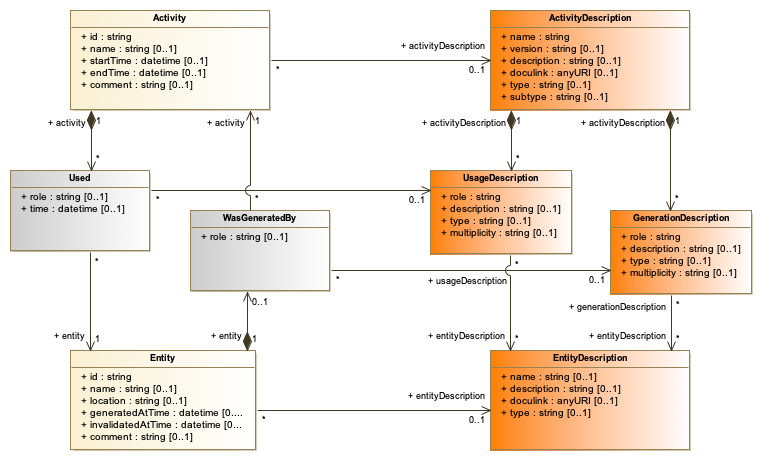
\includegraphics[width=1.0\textwidth]{2019-05-17_IVOAModel_VODML_Descriptions.png}
\caption[Partial class diagram focused on description classes.]{Partial class diagram focused on description classes.}
\label{fig:classdiagram_descriptions}
\end{figure}

% \begin{figure}[ht]
% \centering
% 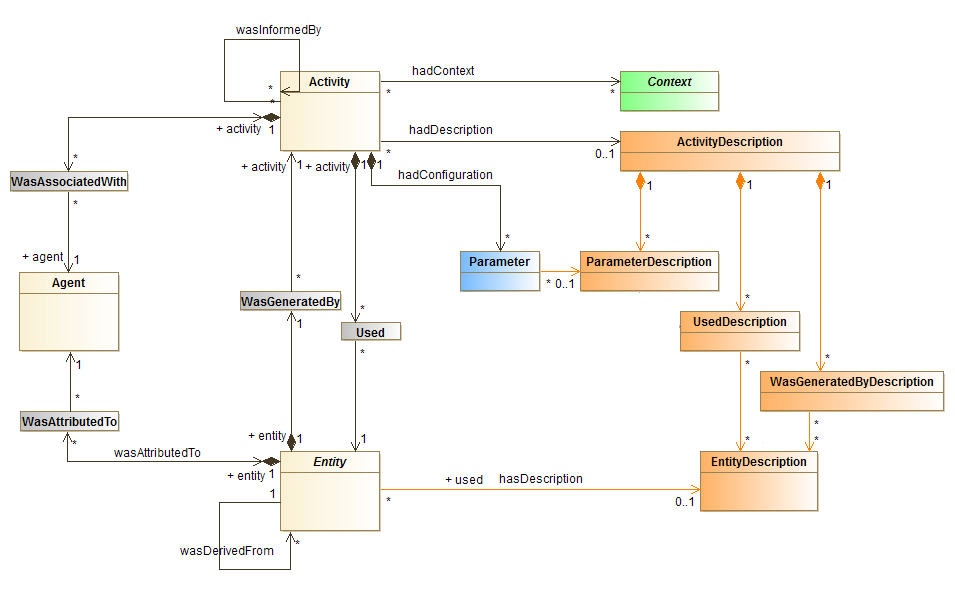
\includegraphics[width=1.0\textwidth]{ExtendedModel_VODML_2018-10-10.png}
% \caption[VO-DML compatible version of the class diagram in Figure~\ref{fig:classdiagram}]{VO-DML compatible version of the class diagram in Figure~\ref{fig:classdiagram}.}
% \label{fig:classdiagram_vodml}
% \end{figure}


% 2018-12 commented
%A similar normalization of descriptions of the actual processes and datasets can be found in the IVOA Simulation DM \citep[SimDM, ][]{std:SimDM}), which describes simulation metadata. The SimDM classes \class{Experiment} and \class{Protocol} correspond to the Provenance terms \class{Activity} and \class{ActivityDescription}.


% 2018-09 commented
% %The association
% %classes for the many-to-many relations are modelled as mapping classes.
% When implementing the model in a relational database, the many-to-many relations can be
% represented as individual tables for mapping the relation. We model one of each
% of the associations of the many-to-many relationships as a composition (full
% diamond) if the mapping class belongs more strongly to one of its linked
% classes; e.g. the \emph{Used} relations are strongly dependent on the
% corresponding \emph{Activities}. 



\subsubsection{ActivityDescription class}
\label{sec:activity_desc}


\begin{table}[ht]
\small
\tymax  0.5\textwidth
\textbf{\normalsize ActivityDescription}\vspace{0.25em}\\
\begin{tabulary}{1.0\textwidth}{llL}
\toprule
\head{Attribute} &  \head{Data type} & \head{Description}\\
\midrule
%\textbf{id}  & string & a unique id for this activity description\\
\textbf{name}         & string & a human-readable name\\
version      & string & a version number, if applicable (e.g. for the code used)\\
description  & string & additional free text description for the activity\\
doculink     & anyURL & link to further documentation on this activity, e.g. a 
paper, the source code in a version control system etc.\\
type        & string & type of the activity\\
subtype     & string & more specific subtype of the activity\\
% code         & string & the code (software) used for this process, if applicable\\
\bottomrule
\end{tabulary}
\caption[Attributes of the \class{ActivityDescription} class]{Attributes of the \class{ActivityDescription} class. Attributes in \textbf{bold} must not be null.
%Some of the attributes inherited from Entity (see Table~\ref{tab:entity}) are not indicated in this table.
}\label{tab:activitydescription}
\end{table}


How an activity works internally is further explained by information contained in the \class{ActivityDescription} class.
% This could be, for instance, the name of the \attribute{code} and its \attribute{version} used to perform an activity or a more general description of the underlying algorithm or process. 
An activity is then a concrete case (instance) with a given start and stop time, and it refers to a description for further information.

%A close concept in the W3C PROV-DM is the \class{Plan} (defined as a subclass of \class{Entity}). However a plan in PROV-DM is primarily attached to the \class{Agent} class with \class{hadPlan} through the \class{wasAssociatedWith} relation. It is accepted to omit the agent, but it is always supposed that an agent exist.
\class{ActivityDescription} is directly attached to \class{Activity} and can thus be seen as a list of attributes that can be known before an \class{Activity} instance is created. 

There must be exactly zero or one \class{ActivityDescription} per \class{Activity}. 
% If steps from a pipeline shall be grouped together, one needs to create a proper \class{ActivityDescription} for describing all the steps at once. This method can then be referred to by the pipeline activity. 

The activity \attribute{type} is a free text attribute, but if one of the terms in Table \ref{tab:activitydescription} applies, it should be used.
%except for predefined words listed in Table \ref{tab:activitydescription-roles}.
The activity \attribute{subtype} is a free text attribute to be used internally by the project that defined \class{ActivityDescription} instances (e.g. mosaicing, denoising, photometric calibration, cross correlation).

%predefined words listed in a dedicated vocabulary webpage.

% examples : observation, simulation; regridding, fusion, calibration, reconstruction (WD 2018)
% data acquisition (observation or simulation), reduction, calibration, publication
% selection, calibration, analysis


\begin{table}[ht]
\small
\tymax  0.5\textwidth
\textbf{\normalsize ActivityDescription types}\vspace{0.25em}\\
\begin{tabulary}{1.0\textwidth}{lL}
\toprule
\head{Type} & \head{Comment} \\
\midrule
Observation    & Active acquisition of information on a phenomenon\\
Simulation     & Generation of data through a computational process\\
Reduction      & Transformation of digital information into a corrected, ordered, and simplified form\\
Calibration    & Transformation and comparison of measurement values with respect to a calibration standard of known accuracy\\
Reconstruction & Estimation of physical properties using indirect information\\
Selection      & Application of filters or criteria to select partial information\\
Analysis       & Process of inspecting, cleansing, transforming, and modeling data with the goal of discovering useful information, informing conclusions, and supporting decision-making\\
\bottomrule
\end{tabulary}
\caption[Terms applicable as activity types.]{Terms applicable as activity types.}
\label{tab:activitydescription-roles}
\end{table}




\subsubsection{EntityDescription class}
\label{sec:entity_desc}


\begin{table}[ht]
\small
\tymax  0.5\textwidth
\textbf{\normalsize EntityDescription}\vspace{0.25em}\\
\begin{tabulary}{\textwidth}{llL}
\toprule
\head{Attribute} & \head{Data type} & \head{Description}\\
\midrule
%\textbf{id} & string & a unique identifier for this description\\
name       & string & a human-readable name for the entity description\\
description  & string & a descriptive text for this kind of entity\\
doculink    & anyURL & link to more documentation\\
type      & string & type of the entity\\
% \midrule
% \multicolumn{3}{@{}l}{\textbf{Optional attributes:}} \\
% content\_type    & string & MIME type for the content of the entity\\
% format    & string & type of container for the entity\\
% removed the obscore attributes, since specific for observations only, not applicable to configuration entities etc.
% dataproduct\_ type  & string       & from ObsCore data model \citep{std:ObsCore}, if applicable; describes, what kind of product it is (e.g. image, table)\\
% dataproduct\_ subtype & string       & from ObsCore data model, more specific subtype\\
% level       & enum integer & the level of processing or calibration; for ObsCore's calib\_level it is an integer between 0 and 3\\
%\midrule
%\multicolumn{4}{@{}l}{\textbf{Additional attributes:}} \\
%\multicolumn{4}{@{}l}{Further project-specific attributes (e.g. format, content\_type) and/or attributes}\\
%\multicolumn{4}{@{}l}{from other data models (e.g. dataproduct\_type and -\_subtype, version, calibLevel}\\
%\multicolumn{4}{@{}l}{from DatasetDM) can be added (Section~\ref{sec:dataset-obscore}).}\\
\bottomrule
\end{tabulary}
\caption[Attributes of the \class{EntityDescription} class]{Attributes of the \class{EntityDescription} class. Attributes in \textbf{bold} must not be null. 
%For simple use cases, this description class may be ignored and its attributes may be used for \class{Entity} instead.
%The utypes may vary depending on the data model, e.g. for simulation data they 
%would point to utypes of SimDM.
}\label{tab:entitydescription}
\end{table}


%The Entity class can have an EntityDescription class attached. 
%The category of entities can be predefined using a description class. 
The \class{EntityDescription} class is meant to store descriptive information for different categories of entities. It contains information that is known before an \class{Entity} instance is created. The \class{EntityDescription} general attributes are summarized in Table~\ref{tab:entitydescription}.

For example, a specific category of entities in a project may be defined in details in a document or on a webpage (e.g. a CTA DL3 file, a CCD device, a photographic plate).

The entity \attribute{type} is a free text attribute, that contains the general category of the entity, e.g. if it is data, a document, a vizualization, a device...

%For example, a format (e.g. JPG images, FITS, FITS-LDAC, \ldots) can be common to several entities. However, the size of this image or file cannot be known before it is created. In this example, format would be an \class{EntityDescription} attribute, while size would be a property attached to the \class{Entity} instance. 

%Additional attributes that describe the content of a dataset could be derived from the Dataset Metadata Model (see Section \ref{sec:dataset-obscore})

The \class{EntityDescription} class should not contain information about the usage of the data, in particular, it generally tells nothing about them being used as input or generated as output. This kind of information should be provided by the relations (and their descriptions) between activities and entities (see Sections~\ref{sec:entity-activity-relations} and \ref{sec:use_gen_desc}).


\subsubsection{UsageDescription and GenerationDescription classes}
\label{sec:use_gen_desc}

\begin{table}[ht]
\small
\tymax  0.5\textwidth
\textbf{\normalsize UsageDescription}\vspace{0.25em}\\
\begin{tabulary}{1.0\textwidth}{llL}
\toprule
\head{Attribute} &  \head{Data type} & \head{Description}\\
% \midrule
% $\rightarrow$ \textbf{activityDescription} & link & link to \class{ActivityDescription}\\
% $\rightarrow$ entityDescription & link & link to \class{EntityDescription}\\
% If we really need the link to EntityDescription, it should be a m:n relation, since there may be UsedDescriptions that accepts more than one type of entity: f.e. a PNG or a FITS file.
% Analogous for the WasGeneratedByDescription; the same Activity may generate different types of files with the same role ("--format=png" or "--format=eps").
\midrule
%\textbf{id} & string & identifier\\
\textbf{role} & string   & function of the entity with respect to the activity \\
description  & string & a descriptive text for this kind of usage \\
type    & string   & type of relation, see Section~\ref{sec:ugtypes} \\
multiplicity & string & Number of expected input entities to be used with the given role. A * indicates that the number of input entities can be more than 1. \\
\bottomrule
\end{tabulary}
\caption[Attributes of the \class{UsageDescription} class]{Attributes of the \class{UsageDescription} class. Attributes in \textbf{bold} must not be null.}
\label{tab:usagedescription}
\end{table}


\begin{table}[ht]
\small
\tymax  0.5\textwidth
\textbf{\normalsize GenerationDescription}\vspace{0.25em}\\
\begin{tabulary}{1.0\textwidth}{llL}
\toprule
\head{Attribute} & \head{Data type} & \head{Description}\\
\midrule
%\textbf{id} & string & identifier\\
\textbf{role} & string & function of the entity with respect to the activity \\
description  & string & a descriptive text for this kind of generation \\
type & string   & type of relation, see section \ref{sec:ugtypes} \\
multiplicity & string & Number of expected output entities that will be generated with the given role. A * indicates that the number of output entities can be more than 1. \\
% \midrule
% $\rightarrow$ \textbf{activityDescription} & link & link to an \class{ActivityDescription}\\
% $\rightarrow$ entityDescription & link & link to \class{EntityDescription}\\
\bottomrule
\end{tabulary}
\caption[Attributes of the \class{GenerationDescription} class]{Attributes of the \class{GenerationDescription} class. Attributes in \textbf{bold} must not be null.}
\label{tab:wasgeneratedbydescription}
\end{table}


In order to describe more precisely an activity, the expected inputs and outputs of this activity should be specified.

% 2018-12 commented
% In the case of workflow description models, such as ProvONE (but also Kepler or Taverna for example), input and output \textbf{ports} are defined, and can be connected to build a workflow of activities. In ProvONE \citep{ProvONE}, an \class{ActivityDescription} is restricted to a \class{Program}, and an \class{Activity} is an \class{Execution} associated to a \class{Program}, with further entities and relations dedicated to workflow descriptions (see Section\ref{sec:dmlinks}). However, the description of workflows is out of the scope of this document, and the more general concepts we introduce here are the UsedDescription and the WasGeneratedByDescription classes. Those classes are meant to store descriptive information about the usage or generation of an entity that is known before the activity is executed.

We introduce the \class{UsageDescription} and the \class{GenerationDescription} classes, that are meant to store the information about the usage or generation of entities that is known before an activity instance is executed, i.e. what we expect to store in the \class{Used} and \class{WasGeneratedBy} relations (see \ref{sec:entity-activity-relations}). 
Instances of \class{Used} (respectively \class{WasGeneratedBy}) may thus point to an instance of \class{UsageDescription} (respectively \class{GenerationDescription}).

%The \attribute{role} value given in the \class{UsageDescription} (respectively \class{GenerationDescription}) should correspond to the \attribute{role} value of the related \class{Used} (respectively \class{WasGeneratedBy}). See \ref{sec:roles}.

If a \class{UsageDescription} (respectively \class{GenerationDescription}) instance is defined, the \attribute{role} attribute of the related \class{Used} (respectively \class{WasGeneratedBy}) instances must match the \attribute{role} attribute of this \class{UsageDescription} (respectively \class{GenerationDescription}) instance.

A \attribute{multiplicity} attribute  should be specified to indicate the number of entities expected to share the same role, e.g. in the case of the stacking of images, several images are expected with the same input role (\attribute{multiplicity=*}).

When related to the \class{UsageDescription} or \class{GenerationDescription}, the attributes of \class{EntityDescription} (see Section~\ref{sec:entity_desc}) help to describe the category of entities expected as an input or an output in an activity. For example: the input bias files must be in FITS format (relation to a \class{DatasetDescription} with \attribute{contentType}=application/fits), or the red, green and blue channel images must be in PNG or JPEG format. 


\subsubsection{Types of Usage and Generation}
\label{sec:ugtypes}

The typing of those relations is particularly needed to enable quality assessment and identification of error sources in the process (see goals C and D in Section \ref{sec:goals}), so as to facilitate the exploration of provenance information. 

The type of usage or generation is an optional attribute.
%For example
It is a free text attribute, but if one of the terms in Table \ref{tab:usage-generation-types} applies, it should be used.
%except for predefined words listed in Table~\ref{tab:usage-generation-types}. 

The type "main" indicates the main input and output entities of an activity. It should help to provide the minimum relevant data flow to the initial entity or activity, i.e. to find the most relevant progenitors.

\begin{table}[ht]
\small
\tymax  0.5\textwidth
\begin{tabulary}{1.0\textwidth}{Lp{9cm}}
\toprule
\head{Type} & \head{Description} \\
\midrule
Main           & main input or output entities of the activity, i.e. strictly necessary, and the primary objective of the activity.\\
Calibration    & usage of an entity to calibrate another entity.\\
Preview        & generation of a quick representation of an entity.\\
Setup          & usage of an entity as configuration information, see also Section~\ref{sec:configurationpackage}\\
Quality        & generation of information that helps to assess the quality of the activity results, example: errors, warnings, flags, percentage of overexposed pixels, ...\\
Log            & generation of logging information \\
Context        & contextual information that influences the activity, but for which there are no or little control at the moment of its execution, examples: temperature, wind, conditions of observation, execution platform, operating system, instrumental context, ...\\
\bottomrule
\end{tabulary}
\caption[Terms applicable as usage or generation type.]{Terms applicable as usage or generation type.}
\label{tab:usage-generation-types}
\end{table}



\subsection{Specific types of Entity classes}
\label{sec:spec_entities}

\class{Entity} and \class{EntityDescription} classes carry the minimum metadata that can apply to any kind of entity without specifying the nature or the structure of the content of the entity. 
In some cases, the structure of the content is relevant information to assess the usefulness of the entity, in particular for datasets.

In some other cases, the content itself of an entity is relevant information to assess the usefulness of the related entities or activities. Such content must then be expose as properly described values.

In astronomy and the VO, we thus define two main types of entity classes:

\begin{itemize}
    \item \textbf{Dataset}: a dataset is a resource which encodes data in a defined structure. It is generally a file or a set of files which are considered to be a single deliverable. The content may be e.g. a cube, an image, a table, a list.
    \item \textbf{Value}: a value is an atomic piece of data with a given value type (e.g. a data type such as boolean, integer, real, string).
\end{itemize}


\begin{figure}[ht]
\centering
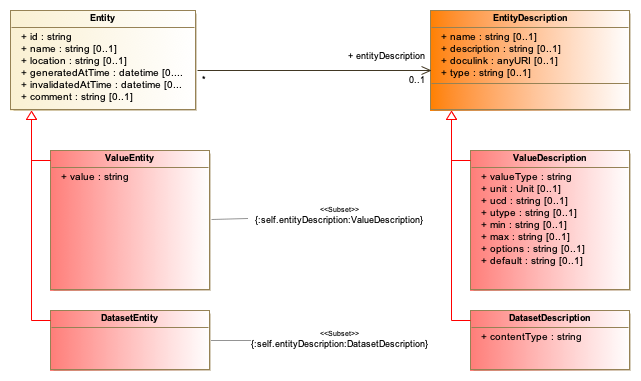
\includegraphics[width=1.0\textwidth]{figures/2019-05-17_IVOAModel_VODML_EntityClasses.png}
\caption[Partial class diagram focused on specific types of Entity classes.]{Partial class diagram focused on Specific types of Entity classes.}
\label{fig:classdiagram_entityclasses}
\end{figure}

We anticipate that more specific categories of entities can be defined by the projects (for example, a Device, a Document, a Vizualization...). The \attribute{type} attribute of the \class{EntityDescription} class should be used to differentiate the different categories of entities.


\subsubsection{DatasetEntity and DatasetDescription classes}

The handling of datasets is implemented in the model by a \class{DatasetEntity} class. A corresponding \class{DatasetDescription} class contains a \attribute{contentType} attribute that must not be null (see Table~\ref{tab:datasetdescription}).

The \attribute{contentType} may indicate the MIME-type or format of a file, or a more precise structure, following the definition of the attribute \attribute{access\_format} defined in ObsCoreDM (\citet{std:OBSCORE}, Section 4.7).

\begin{table}[ht]
\small
\tymax  0.5\textwidth
\textbf{\normalsize DatasetDescription}\vspace{0.25em}\\
%\begin{tabulary}{1.0\textwidth}{@{}p{2.5cm}p{0cm}lL@{}}
\begin{tabulary}{1.0\textwidth}{llL}
\toprule
\head{Attribute} &  \head{Data type} & \head{Description}\\
\midrule
\textbf{contentType}  & string  & MIME-type or format of the dataset \\
\bottomrule
\end{tabulary}
\caption[Attributes of the \class{DatasetDescription} class]{Attributes of the  \class{DatasetDescription} class. The class also inherits the attributes of \class{EntityDescription} listed in Table \ref{tab:entitydescription}. Attributes in \textbf{bold} must not be null.}
\label{tab:datasetdescription}
\end{table}


\subsubsection{ValueEntity and ValueDescription classes}

The handling of values is implemented in the model by a \class{ValueEntity} class that contains a \attribute{value} attribute. A corresponding \class{ValueDescription} class contains attributes commonly used in the VO to qualify values. Those attributes are listed in Table~\ref{tab:valuedescription}.

\begin{table}[ht]
\small
\tymax  0.5\textwidth
\textbf{\normalsize ValueDescription}\vspace{0.25em}\\
%\begin{tabulary}{1.0\textwidth}{@{}p{2.5cm}p{0cm}lL@{}}
\begin{tabulary}{1.0\textwidth}{p{2cm}LL}
\toprule
\head{Attribute} &  \head{Data type} & \head{Description}\\
\midrule
%\textbf{id}  & string & parameter unique identifier\\
\textbf{valueType} & string & VODML value type, see \citet{std:VODML} \\
unit        & string & physical unit, see \citet{std:VOUNIT} for recommended unit representation \\
ucd         & string  & Unified Content Descriptor, supplying a standardized classification of the physical quantity, see \citet{std:UCD}\\
utype       & string  & Utype, meant to express the role of the value in the context of an external data model, see \citet{note:utypeusage} \\
%xtype       & string & extended datatype as in VOTable 1.2 and above. A list of proposed \\
% \midrule
% \multicolumn{3}{@{}l}{\textbf{Optional attributes:}} \\
min         & string whose value can be interpreted by the valueType attribute & minimum value \\
max         & string whose value can be interpreted by the valueType attribute & maximum value\\
options     & string & comma separated list of possible values\\
default     & string whose value can be interpreted by the valueType attribute & the default value of the value entity \\
\bottomrule
\end{tabulary}
\caption[Attributes of the \class{ValueDescription} class]{Attributes of the \class{ValueDescription} class. The class also inherits the attributes of \class{EntityDescription} listed in Table \ref{tab:entitydescription}. Attributes in \textbf{bold} must not be null.}
\label{tab:valuedescription}
\end{table}




\subsection{Activity configuration}
\label{sec:configuration}

Configuring an activity is the way to set parameters so that the activity occurs in the desired conditions.

In some cases developed in Section~\ref{sec:goals} (goals C and D in particular), configuration information is relevant to assess the quality and reliability of an activity or an entity, and to identify the location of configuration errors in a processing. It also facilitates the re-execution of an activity (reproducibility).

Configuration information may be carried by entities using the core features, where an entity (e.g. \class{ValueEntity} and \class{DatasetEntity} instances) is referenced in \class{Used} relations with a given \attribute{role} and \attribute{type}=“setup”. With this solution, the configuration information is independent from the activity and can be generated and used as any entity.

The data model also provides a specialized ActivityConfiguration package to directly attach configuration information to an activity. This package is composed of a \class{WasConfiguredBy} relation connected with \class{Parameter} and \class{ConfigFile} classes (see~\ref{sec:configurationpackage}). With this solution the configuration information is independent from the entities, and seen as part of the activity.

%With the combination of those orientations, a project can select which pieces of configuration information is to be tracked, and which is to be simply attached to an activity.

%In some cases, it may be relevant to define all inputs as entities, following the pattern Activity-Used-Entity. 

%In other cases, it may be relevant to attach configuration information directly and specifically to the activity, and define as entities only the objects that are to be traced.

%Access to configuration and access to provenance information are seen as different features of the model, the ActivityConfiguration part is thus kept separated from the execution and description parts of the model, even though they can have connections. 

%Activity configuration typically implies a set of input parameters attached to the activity before execution, or a configuration file that contains those parameters. In order to link this detailed configuration with provenance information, a \class{Parameter} class is connected to the \class{Activity} class, along with a \class{ParameterDescription} class. 


% Activity Configuration package overview
\begin{figure}[hbt]
\centering
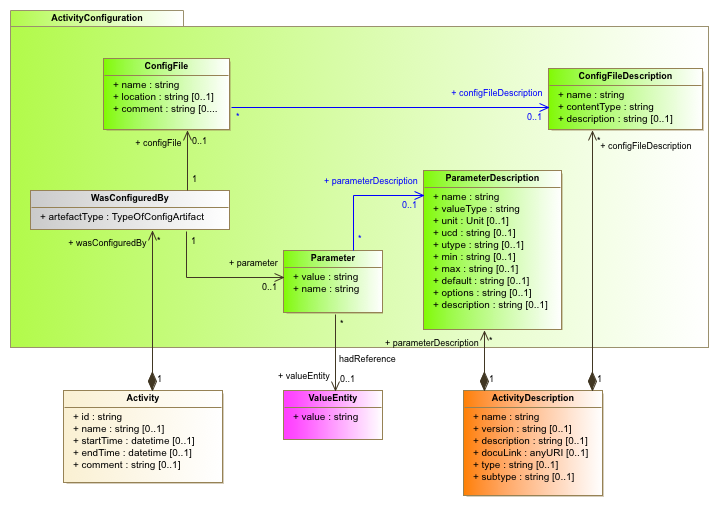
\includegraphics[width=1.0\textwidth]{PROV_Fig7.png}
% Mireille: updated the diagram file for the last version with the proper cardinalities for Parameter and ConfigFile
\caption[Partial class diagram focused on the \class{ActivityConfiguration} package.]{Partial class diagram focused on the \class{ActivityConfiguration package}. The \class{Parameter} and \class{ConfigFile} classes provide configuration information for an \class{Activity} instance. The right side of the diagram shows the descriptions, where an \class{ActivityDescription} class is bound to the \class{ParameterDescription} and \class{ConfigFileDescription} classes.}
\label{fig:activityconfig}
\end{figure}
% classes attributes 


\subsubsection{Overview of the ActivityConfiguration package} \label{sec:configurationpackage}

As shown in Figure \ref{fig:activityconfig} the \class{ActivityConfiguration} package contains two classes for the execution side: \class{Parameter} and \class{ConfigFile} which are connected to an \class{Activity} instance via the \class{WasConfiguredBy} association class.
An \class{Activity} may thus be configured by a set of \class{Parameter} instances, or by \class{ConfigFile} instances containing a list of (key,value) pairs, or by a combination of both. 

% Mathieu: commented as it is about implementation
%The value stored in a \class{Parameter} can be explicitly queried while the values inside a \class{ConfigFile} need a search method for this.  This current standard does not provide the description for search methods and leaves it to the projects. 

The corresponding description classes, \class{ParameterDescription} and \class{ConfigFileDescription}, are both defined in the context of the description of an activity. 
There can be several instances of a \class{Parameter} (respectively \class{ConfigFile}) that are described by the same instance of \class{ParameterDescription} (respectively \class{ConfigFileDescription}).
%, as the activities they configure may refer to the same ActivityDescription instance. 

% Mathieu: commented as it is about implementation
%They are e.g. provided by the pipeline designer and filled in together with the \class{ActivityDescription}. 
%This information can be imported from an external service which stores the documentation of the processing or observation methods applied in the activities of the project. 


\subsubsection{Parameter and ParameterDescription classes}
\label{sec:parameterandD}

%The following attributes are defined to handle a Parameter instance and describe it. 

\begin{table}[ht]
\small
\tymax  0.5\textwidth
 \textbf{\normalsize Parameter}\vspace{0.25em}\\
 \begin{tabulary}{1.0\textwidth}{llL}
 \toprule
 \head{Attribute} & \head{Data type}   & \head{Description}\\
 \midrule
%\textbf{id}   & string            & a unique id\\
\textbf{name}  & string & name of the parameter \\
\textbf{value} & string & the value of the parameter. If a corresponding \class{ParameterDescription}.\attribute{valueType} attribute is set, the value string can be interpreted by this \attribute{valueType}. \\
\bottomrule
\end{tabulary}
\caption[Attributes of the \class{Parameter} class]{Attributes of the \class{Parameter} class. Attributes in \textbf{bold} must not be null.}
\label{tab:param}
\end{table}

\begin{table}[ht]
\small
\tymax  0.5\textwidth
\textbf{\normalsize ParameterDescription}\vspace{0.25em}\\
\begin{tabulary}{1.0\textwidth}{lLL}
 \toprule
 \head{Attribute} & \head{Data type}   & \head{Description}\\
 \midrule
%\textbf{id}  & string &  unique ParemeterDescription identifier\\
\textbf{name} & string & name of the parameter \\
\textbf{valueType} & string & VO-DML value type, see \citet{2018ivoa.spec.0910L} \\
description & string  & a descriptive text for the parameter \\
unit        & Unit  & physical unit, see \ref{sect:Units} and \citet{2014ivoa.spec.0523D} for recommended unit representation \\
ucd         & string  & Unified Content Descriptor, supplying a standardized classification of the physical quantity, see \citet{2018ivoa.spec.0527M} \\
utype       & string  & Utype, meant to express the role of the parameter in the context of an external data model, see \citet{note:utypeusage} \\
% Mireille   removed the reference to the Utype note by Graham and al. not the definition of it but critics instead. 
%xtype         & string & extended datatype as in VOTable 1.2 and above. A list of proposed \\
% \midrule
% \multicolumn{3}{@{}l}{\textbf{Optional attributes:}} \\
min         & string & minimum value as a string whose value can be interpreted by the \attribute{valueType} attribute \\
max         & string & maximum value as a string whose value can be interpreted by the \attribute{valueType} attribute\\
options     & string & comma separated list of possible values\\
default     & string & the default value of the parameter as a string whose value can be interpreted by the \attribute{valueType} attribute \\
\bottomrule
\end{tabulary}
\caption[Attributes of the \class{ParameterDescription} class]{Attributes of the  \class{ParameterDescription} class. Attributes in \textbf{bold} must not be null.}
\label{tab:Paramdescription}
\end{table}

The \class{Parameter} class contains a \attribute{value} and a \attribute{name} attribute that must be set (Table~\ref{tab:param}).

The \class{ParameterDescription} class describes the parameter \attribute{value} attribute similarly to the \class{ValueEntity} and \class{ValueDescription} classes. Those attributes are listed in Table~\ref{tab:Paramdescription}.

If a \class{ParameterDescription} instance is defined, the \attribute{name} attribute of the related \class{Parameter} instances must match the \attribute{name} attribute of this \class{ParameterDescription} instance.


\subsubsection{ConfigFile and ConfigFileDescription classes}

\begin{table}[ht]
\small
\tymax  0.5\textwidth
 \textbf{\normalsize ConfigFile}\vspace{0.25em}\\
 \begin{tabulary}{1.0\textwidth}{llL}
 \toprule
 \head{Attribute} & \head{Data type}   & \head{Description}\\
 \midrule
%\textbf{id}   & string            & a unique id\\
\textbf{name} &  string & a human-readable name for the config file \\
\textbf{location} & string  &  a path to the config file, e.g. a URL \\
comment & string  & text containing comments on the config file  \\
\bottomrule
\end{tabulary}
\caption[Attributes of the \class{ConfigFile} class]{Attributes of the \class{ConfigFile} class. Attributes in \textbf{bold} must not be null.}
\label{tab:configfile}
\end{table}

\begin{table}[ht]
\small
\tymax  0.5\textwidth
\textbf{\normalsize ConfigFileDescription}\vspace{0.25em}\\
\begin{tabulary}{1.0\textwidth}{llL}
 \toprule
 \head{Attribute} & \head{Data type}   & \head{Description}\\
 \midrule
%\textbf{id}  & string &  unique ParemeterDescription identifier\\
\textbf{name}    & string & a human-readable name for the config file \\
\textbf{contentType}  & string  & MIME-type or format of the dataset \\
description     & string  & a descriptive text for the config file \\
\bottomrule
\end{tabulary}
\caption[Attributes of the \class{ConfigFileDescription} class]{Attributes of the  \class{ConfigFileDescription} class. Attributes in \textbf{bold} must not be null.}
\label{tab:configfiledescription}
\end{table}

The \class{ConfigFile} is a text file, where key value pairs are listed as parameters for running an activity. It contains a \attribute{location} and a \attribute{name} that must be set, and a \attribute{comment} attribute (Table~\ref{tab:configfile}).

The \class{ConfigFileDescription} class indicates the format in which the list is provided in a \attribute{contentType} attribute (see Table~\ref{tab:configfiledescription}). 

If a \class{ConfigFileDescription} instance is defined, the \attribute{name} attribute of the related \class{ConfigFile} instances must match the \attribute{name} attribute of this \class{ConfigFileDescription} instance.


\subsubsection{Relations with Activity class}

\begin{table}[ht]
\small
\tymax  0.5\textwidth
 \textbf{\normalsize WasConfiguredBy}\vspace{0.25em}\\
 \begin{tabulary}{1.0\textwidth}{llL}
 \toprule
 \head{Attribute} & \head{Data type}   & \head{Description}\\
 \midrule
%\textbf{id}   & string            & a unique id\\
\textbf{artefactType} &  TypeOfConfigArtefact & string that takes the value "Parameter" or "ConfigFile" to indicate the type of class pointed by the \class{WasConfiguredBy} instance. \\
\bottomrule
\end{tabulary}
\caption[Attributes of the \class{WasConfiguredBy} class]{Attributes of the \class{WasConfiguredBy} class. Attributes in \textbf{bold} must not be null.}
\label{tab:WasConfiguredBy}
\end{table}

The relation of \class{Parameter} and \class{ConfigFile} to \class{Activity} is formalized by a \class{WasConfiguredBy} class. There must be exactly one instance connected to a \class{WasConfiguredBy} instance, either a \class{Parameter} instance or a \class{ConfigFile} instance. The \class{WasConfiguredBy} class contains the attribute \attribute{artefactType} to indicate the type of class pointed by the \class{WasConfiguredBy} instance (see Table~\ref{tab:WasConfiguredBy}).

The life cycle of a \class{Parameter} instance (respectively \class{ConfigFile} instance) is the one of the corresponding \class{Activity} instance. 
The life cycle of a \class{ParameterDescription} instance (respectively \class{ConfigFileDescription} instance) is the one of the corresponding \class{ActivityDescription} instance. 
This means that when an activity is deleted from the provenance repository, its parameters and config files also disappear.

Several activities launched with various possible values for a parameter share the same \class{ParameterDescription} instance. 
For instance, a cube analysis activity with a parameter "nbofChannels" will point to the corresponding instance of \class{ParameterDescription} (\attribute{name} = "nbofChannels", \attribute{ucd} = "meta.number", \attribute{unit} = NULL, \attribute{description} = "Nb of channel used for segmentation"). 
% Mathieu: this part is about implementation
% Other implementation examples are provided together on the RFC page. See \url{https://wiki.ivoa.net/twiki/bin/view/IVOA/ProvFocusAstericsExamples}.

Similarly, we can foresee a number of different \class{ConfigFile} instances used for various instances of an \class{Activity}, which rely on the same \class{ConfigFileDescription} instance bound to the corresponding \class{ActivityDescription} instance. 

%  ??? a deplacer vers la partie Description ?? 
% Mathieu: This suggest a dedicated serialisation of the description, explained in a separate document
%An \class{ActivityDescription} works as a template which binds to the configuration, to the top of the diagram and to the data flow represented in \class{UsageDescription} and \class{GenerationDescription} where the Entities consumed and produced by the ActivityDescription are designated with their role. Such a template can be imported from a project code repository, for instance. 

%Some \class{Parameter} values may have been elaborated from a computation, a process which produced this value and can be part of the provenance information. In this case an \class{Activity} instance exists in the system that did produce a \class{ValueEntity} instance which contains this specific value. 
The \class{Parameter} instance may refer to a \class{ValueEntity} instance using a \textit{hadReference} which gives the origin of this value. 



%We identify three different ways to link configuration information to an activity:
%\begin{itemize}
%\item Declare a parameter set (or each parameter) as an input entity that is used by the activity. \\
%        This also allows tracking the provenance of the parameter further.
%\item Define families of activities, each one with fixed attributes.\\
%        I.e. use different subclasses for activities with different fixed attributes.
%\item Add activity attributes in the form of key-value parameters.
%\end{itemize}

% 2019-03 commented
% The concept of parameter is very general, and already exists in the VO context in different forms, for example as PARAM elements in VOTable \citep{std:VOTABLE}, as POST/GET parameters for web services \citep[see for example][for SODA services]{std:SODA} or as uws:param elements in the UWS pattern \citep{std:UWS}. 
% The Simulation DM also contains a \class{ParameterSetting} class \citep{std:SimDM}.

% 2019-03 commented
% In the context of web service resources, a list of input parameters is written in the form of an IVOA DataLink Service Descriptor \citep{std:DataLink}, a VOTable resource that contains a group of InputParams with PARAM elements. 
% This connection to Service Descriptors is further developped in Section~\ref{sec:description-serialization}.
% For UWS services \citep{std:UWS}, we also find a list of parameters, some of which may carry identifiers referencing another entity. The link to the UWS pattern is further developed in Section~\ref{sec:uws_links} of the Appendix.

% 2018-09 commented
%We note that a parameter can be seen as a simplified entity, though it can only be used by an activity and it has no provenance. In some cases, it may be relevant to define a specific parameter as an entity if its provenance should be traced.

%For example, observations generally require information on \emph{ambient conditions} as well as
%\emph{instrument characteristics}. This contextual data associated with an observation is not directly modelled in the ProvenanceDM. However, this information can be stored as different entities. 
%Alternatively, one could list the instrument characteristics as a set of key-value parameters using the \class{Parameter} class, so that this information is structured and stored with the provenance information (and can thus be queried simultaneously). 

% 2019-03 commented
%For example, in the case of a processing activity that cleans an image with a sigma-clipping method, the input and output images would be dataset entities and the value of the number of sigma for sigma-clipping would be carried by a \class{Parameter} value set before running the activity. The corresponding \class{ParameterDescription} defines the type and range of the expected value for this parameter (using the attributes \attribute{valueType}, \attribute{min}, \attribute{max}, \attribute{options}...).

%\paragraph{Input parameters for an .}

%\class{UsedDescription} + \class{ParameterDescription} can be seen as a specialized input port attached to an \class{ActivityDescription}. 
%An activity may expect a list of input parameters directly connected to the activity, each one directly described with the attributes of \class{ParameterDescription} as defined in Section~\ref{sec:parameters}. 
%\class{ParameterDescription} has a \attribute{name} attribute that should correspond to the \attribute{role} attribute of \class{UsedDescription}.
%Such a list of input parameters already exist in the IVOA ecosystem for service resources. In this context, they are written in the form of an IVOA DataLink Service Descriptor \citep{std:DataLink}.
